
%----------------------------------------------------------------------------------------------------------------------------------------

% définit le type de document et ses options
\documentclass[a4paper,10pt]{article}

% des paquetages indispensables, qui ajoutent des fonctionnalites
\usepackage[utf8]{inputenc}
\usepackage{graphicx}
\usepackage{lscape}
\usepackage{url}
\usepackage{xspace}
\usepackage[francais]{babel}
%\usepackage{fullpage}

\pagestyle{plain}


%----------------------------------------------------------------------------------------------------------------------------------------


% le debut du contenu
\begin{document}


%----------------------------------------------------------------------------------------------------------------------------------------


%%%%%%%%%%%%%%%%%%%%%%%%%%%%%%%%%%%%%%%%%%%%%%%%%
%%Page d'accueil
\begin{center}
	%%
	\hspace{3cm}
	
\includegraphics[scale=0.8]{logo.ps}

	%%
	\vspace{1cm}
	{\large Projet de spécialité 2010}\\
	{\Large Conception d'un modèle de feu 3D temps réel}\\
	\vspace{1cm}


	\includegraphics[scale=0.3]{feu.ps}\\
	\vspace{2cm}
	%%
	Etudiants impliqués :\\
	Benjamin Aupetit - IRVM - benjamin.aupetit@ensimag.imag.fr\\
	Julien Champeau - IRVM - julien.champeau@ensimag.imag.fr\\
	Arnaud Emilien - IRVM - arnaud.emilien@ensimag.imag.fr\\
	~\\
	Encadrants :\\
	Marie-Paule Cani  -  Marie-Paule.Cani@inrialpes.fr \\
	Aurélie Catel - aurelie.catel@grenoble-inp.fr
	~ \\
	\vspace{3mm}
	Ensimag 2010\\

\end{center}


\newpage

\tableofcontents

\newpage



%----------------------------------------------------------------------------------------------------------------------------------------
%%%%%%%%%%%%%%%%%
\section{Présentation du projet}
\subsection{Introduction}

\subsection{Objectifs initiaux}
Le but principal de notre projet est de modéliser du feu en temps
réel. Cette modélisation devra être la plus réaliste possible, en
effet nous voulons permettre d'integrer notre solution dans un
environnement temps réel qui requiert un comportement proche de la
réalité en restant intéractif. Dans ce sens notre solution ne sera pas
adaptée à tous les jeux videos, car ceux ci ne necessitent pas une
approche réaliste mais juste des effets visuels impressionants.\\

Notre solution devra ainsi répondre aux critères suivants :
\begin{itemize}
\item Modèle de flamme convainquant 
\item Génération de fumée
\item Propagation réaliste sur l'objet 
\item Prise en compte des flux d'air ( vent, advection du feu... )
\item Destruction procedurale progressive d'un objet
\item Propagation à l'environnement
\end{itemize}

\subsection{Aperçu}

%%%%%%%%%%%%%%%%%
\section{Aperçu de notre modèle}
Ici nous présentons un résumé de notre modèle global. Ce modèle a été
établi pour avoir un idée générale et ainsi choisir les modèles
adaptés pour chaque parties. En effet nous devons nous assurer de la
compatibilité de ceux ci, pour eviter les incohérences entre les
différentes étapes, ou des calculs de syncrhonisation entre les
phases. Par exemple la représentation des objets doit être définié dès
le début mais aussi permettre toutes les opérations que nous pourrions
être amenné à y apporter.

\subsection{Les flammes}
Pour modéliser les flammes il faut différencier deux aspects. Le rendu
des flammes d'une part, et la modélisation du phénomène associé
d'autre part.

\subsubsection{Un modèle de fluide pour le feu}
Basé sur les travaux de \textbf{Jos Stam} (stable fluids). Ce modèle inclu la
diffusion de la densité, la chaleur, la vitesse des fluides utilisés (
``combustible'', fumée, air ). Il permettra aussi de gerer plus
simplement la diffusion du feu dans l'environnement.

\subsubsection{Le rendu des flammes et de la fumée}
Pour rendre les flammes nous avons besoin d'une méthode rapide mais
donnant une impression de réalisme. Pour faire ceci nous utilisons une
méthode expliquée \textbf{Zeki Melek}. Cette méthode consiste à
découper le fluide en ``tranches'' othogonale à l'orientation de la
camera. Dans chaque tranche on calcule une texture d'après la densité
de fluide représentant la flamme. Ensuite avant le rendu on applique
un bruit de Perlin ( en 4D ) sur chaque tranche, et enfin on applique
un effet de ``bloom'' sur chaque texture pour modéliser la luminosité
du feu. De plus nous appliquons une couleur à la flamme qui est fonction de 
sa chaleur ( principe du corps noir ).\\
La fumée sera rendue de la même manière que la flamme.

\subsection{Les objets}
Dans un premier temps nous nous concentrerons sur des objets qui se
décomposent lors de la combustion. Pour cela nous utilisons une
décomposition tétrahédrale des maillages des objets pour les
décomposer. Cette méthode permet en effet de détruire localement les
maillages en conservant la géometrie locale des objet (si elle ne
brule pas).



\section{Analyses Bibliographiques}
%%%%%%%%%%%%%%%%%
Cette section regroupe les différents articles lus, concernant les travaux déjà effectués dans ce domaine. 
Nous allons expliquer brièvement de quoi ils parlent, ce que nous en avons retenu de bien ou de mal, ce que nous allons 
utiliser...

\subsubsection{Real-Time Fluid Dynamics for Games}
\textbf{Auteur(s)} : Jos Stam.\\
\textbf{Publication} : Proceedings of the Game Developer Conference, March 2003 \\
\textbf{Sujet(s) abordé(s)} : \\
    Modèle de fluide temps réel, pouvant être utilisé pour le feu, la fumée\\
	Le modèle gère: le deplacement du fluide, la gestion de combustible,les forces appliquées sur le fluide.\\	
\textbf{Principe} :\\
	Le modèle a été décomposé sur plusieurs étapes : génération du fluide par des sources, ajout des forces, diffusion du fluide, puis résolution de l'équation de la densité et de l'équation de la vitesse (équations de Navier-Stockes).
	Pour résoudre les deux équations, il utilise une astuce permettant de résoudre le système très rapidement.
	Enfin, il utilise le principe de conservation de la masse, qui rajoute des effets réalistes de vortex, avec la décomposition de Hodge.\\
\textbf{Point(s) positif(s)} :\\
	Temps réel.\\
	C'est facile à implémenter (moins de 100 lignes pour la version 2D)\\
	Peut être adapté pour la propagation du feu.\\
	Peut être adapté pour qu'un objet influe sur le modèle.\\
	Résultat réellement joli et réaliste.\\
	Très bien expliqué.\\
	Il a fournit un exemple 2D pour de la fumée, plutôt impréssionant.\\
	Le modèle peut s'adapter au feu, à la fumée, et à l'eau.\\
\textbf{Point(s) négatif(s)} :\\
	La zone d'influence est assez petite, il faut voir si c'est possible de l'étendre sans trop allourdir les calculs. (Octree?) \\
	Pas trop de détails sur la représentation graphique du feu.\\	
	La dissipation numérique implique que le résultat n'est pas exact.\\
\textbf{Conclusion} :\\
	C'est sans doute ce que nous allons adapter, pour qu'il serve à la fois pour le feu, la fumée, et la propagation.

\subsubsection{Stable Fluids}
\textbf{Auteur(s)} : Jos Stam.\\
\textbf{Publication} : SIGGRAPH 99 Conference Proceedings\\
\textbf{Sujet(s) abordé(s)} : \\
Résolution de l'équation des fluides ( Navier-Stockes) avec, pour la première fois, un algorithme inconditionnellement stable.\\
\textbf{Principe} :\\
C'est une résolution de Navier-Stockes orientée "Computer Graphic", dans le sens o`u la résolution n'est pas exacte, et ne serait pas utilisable pour des vraies simulations de fluides, mais est "graphiquement adaptée" au problème de fluides.\\
Résolution en quatre étapes : ajout des forces, advection, diffusion, conservation de la masse.\\
\textbf{Point(s) positif(s)} : \\
2D et 3D.\\
Facile à implémenter.\\
Résolution stable et temps réel.\\
Résultat réaliste.\\
\textbf{Point(s) négatif(s)} :\\
La dissipation numérique implique que le résultat n'est pas exact.\\
\textbf{Conclusion} :\\
Ce modèle de fluide semble le plus adapté si nous choisissons d'utiliser un modèle de fluide pour le feu, la fumée et la propagation.


\subsubsection{An Interactive Simulation Framework for Burning Objets}
\textbf{Auteur(s)} : Zeki Melek, John Keyser.\\
\textbf{Publication} : Technical Report 2005 3 1, Texas AM Department of Computer Science, 2005. \\
\textbf{Sujet(s) abordé(s)} : \\
Premier modèle essayant de réaliser en même temps une propagation
de feu réaliste avec un modèle de fluide, de la propagation sur un objet et entre les objets, et de la destruction
d'objets.\\
\textbf{Principe} :\\	
Le modèle de fluide utilise Stable Fluid de \textbf{Stam}. \\
\textbf{Point(s) positif(s)} :\\
    Temps réel\\
    Modèle de fluide, propagation, gestion des objets, destruction des objets.\\
\textbf{Point(s) négatif(s)} :\\
    L'implémentation CPU est lente ( 4fps pour une grille 20*20*20 )\\      
\textbf{Conclusion} :\\


\subsubsection{Visual Simulation of Smoke}
\textbf{Auteur(s)} : Ronald Fedkiw, Jos Stam, Henrik Wann Jensen.\\
\textbf{Publication} : SIGGRAPH 2001 Conference Proceedings \\
\textbf{Sujet(s) abordé(s)} : \\
	Création d'un modèle de fumée, basé sur le travail de Stam ( Stable Fluids ).\\
	Rendu réaliste de la fumée.\\
\textbf{Principe} :\\	
	L'équation du fluide est résolue comme dans "Stable Fluids". Cette fois la chaleur est prise en compte, et traitée de la même manière que la densité. Il en résulte une force de préssion qui s'ajoute simplement au modèle. Le modèle prend en compte les petits phénomènes de vortex qui se créent dans le fluide, basée sur la méthode de Steinhoff ("Vorticity confinement"). Ainsi ils rajoutent une force de rotation pour créer les minis vortex.\\
Pour le rendu : ils découpent la grille de voxels en plusieurs plans, rendus comme une superposition de plans transparents.
Une autre méthode de rendu, plus réaliste, utilise une méthode de lancé de rayons.\\
\textbf{Point(s) positif(s)} :\\
	Gestion de la chaleur.\\
	Rendu très réaliste de la fumée.\\
\textbf{Point(s) négatif(s)} :\\
	Pas en temps réel.\\
\textbf{Conclusion} :\\
	La méthode de rendu semble interessante. De plus la création de minis vortex est un atout pour le côté réaliste du modèle.
	

\subsubsection{Simulating Water and Smoke with an Octree Data Structure}
\textbf{Auteur(s)} : Frank Losasso, Frédéric Gibou, Ron Fedkiw.\\
\textbf{Publication} : SIGGRAPH 2004\\
\textbf{Sujet(s) abordé(s)} : \\
	Simulation d'eau et de fumée. L'équation de Navier-Stockes est résolue sur une grille Octree.\\
	La grille du modèle de fluide s'adapte selon le niveau de détail du phénomène ( par exemple plus de détails là o`u il y a des minis vortex)\\
\textbf{Principe} :\\	
	Le calcul de l'équation des fluides est effectué sur un Octree.\\
\textbf{Point(s) positif(s)} :\\
	L'octree n'est pas restreint ( ce qui était le cas des travaux précédents ).\\
	Réduction des calculs de 75\% pour un résultat équivalent avec une grille à pas constant.\\
\textbf{Point(s) négatif(s)} :\\
	Pas temps réel.\\
	Compliqué à mettre en place.\\
\textbf{Conclusion} :\\
	La complexité de la programmation est assez importante. L'avantage de cette méthode est d'avoir un très haut niveau de détail en effectuant plus de calculs là o`u cela est nécessaire. La précision que nous désiront n'est peut être pas suffisante pour nécessiter un tel modèle.



\subsubsection{Real-Time Simulation of Deformation and Fracture of Stiff Materials}
\textbf{Auteur(s)} : Matthias Müller, Leonard McMillan, Julie Dorsey, Robert Jagnow.\\
\textbf{Publication} : EUROGRAPHICS 2001 Computer Animation and Simulation Workshop \\
\textbf{Sujet(s) abordé(s)} : \\
	Destruction réaliste et temps réel d'un objet. \\
\textbf{Principe} :\\	
	C'est la simplification d'un problème de propagation en négligeant les effets microscopiques, qui ne sont pas vraiment visibles en temps réel, mais coûtent énormement en calcul.\\
	Les meshs sont représentés par des "tetrahedral meshes". Le modèle de propagation continu est transformé en modèle discret. L'élasticité des objets est prise en compte.\\
\textbf{Point(s) positif(s)} :\\
	Temps réel.\\
	Le système est stable est rapide.\\
	La méthode de destruction de l'objet basée sur des tétrahèdres est très intéressante.\\
	Propagation des effets de la destruction à l'intérieur de l'objet.\\
\textbf{Point(s) négatif(s)} :\\
	Peut être lourd à utiliser si il y a trop d'objets à l'écran.\\
\textbf{Conclusion} :\\
	Le principe de déformation sur un mesh tétrahédral est très intéressant, et peut facilement s'adapter à un modèle de fluide.


\subsubsection{Voxels On Fire}
\textbf{Auteur(s)} : Ye Zhao, Xiaoming Wei, Zhe Fan, Arie Kaufman, Hong Qin.\\
\textbf{Sujet(s) abordé(s)} : \\  Animation et propagation de flammes, avec brulure de l'objet.\\
\textbf{Principe} :\\ L'animation et la propagation sont gérés par un modèle de fluide ( Lattice Boltzmann Model ), avec une grille régulière. L'objet est représenté sous forme de voxels, sur lequel est calculé un champs de distance. Le voxel de l'objet est considéré comme un combustible. Pour le rendu ils utilisent des particules et le splatting ( \textbf{Westover} ).\\
\textbf{Point(s) positif(s)} :\\
    - temps réel ( 24fps pour une grille 64*64*64)\\
    - propagation réaliste\\
    - l'objet est brulé progressivement\\
\textbf{Point(s) négatif(s)} :\\
    - le rendu utilise un grandn ombre de particules pour être réaliste\\
    - l'objet n'est pas détruit seule la texture est altérée\\
\textbf{Conclusion} :\\

\subsubsection{Meshes On Fire}
\textbf{Auteur(s)} : Haeyoung Lee, Laehyun, Mark Meyer, Mathieu Desbrun.\\
\textbf{Publication} : Eurographics Workshop on Computer Animation and Simulation '2001 \\
\textbf{Sujet(s) abordé(s)} : \\
	Propagation des flammes à la surface d'un objet.\\
\textbf{Principe} : \\
	La propagation est un parcours géodésique de la surface, et subit le vent environnant.\\	
	Les flammes sont rendues sont formes de particules avec des blobs.\\
	Les flammes générées subissent le champ de vent ce qui les rend plus réaliste.\\
\textbf{Point(s) positif(s)} :\\
	Temps réel.\\
	Prise en compte de plusieurs feu.\\
	Rapide à calculer.\\
	Très efficace pour changer la texture d'un objet brulé.\\
	Propagation fonction d'un champ de vent.\\
	Les particules de feu générées peuvent être utilisées pour génerer un feu 
	sur un autre objet ou sur une autre partie de l'objet.\\
\textbf{Point(s) négatif(s)} :\\
	Ne peut pas s'adapter à la destruction d'un objet.\\
	Peut être une perte de performance si on utilise les particules de feu pour 
	allumer des foyer aux autres endroits du mesh.\\
	La propagation surfacique n'est pas toujours adaptés.\\	
\textbf{Conclusion} :\\
	Ce modèle est interessant, mais nécessite d'être beaucoup modifié pour 
	correspondre à notre but. Il n'est pas très adapté à la destruction des objets. 
	(Sauf si nous voulons uniquement dégrader la texture de l'objet) \\

\subsubsection{Real-time Procedural Volumetric Fire}
\textbf{Auteur(s)} : Alfred R. Fuller, Hari Krishnan, Karim Mahrous, Bernd Hamann, Kenneth I. Joy.\\
\textbf{Publication} : Proceedings of the 2007 symposium on Interactive 3D graphics and games\\
\textbf{Sujet(s) abordé(s)} : \\
	Rendu de feu réaliste en temps réel, utilisant le bruit de perlin.
\textbf{Principe} :\\
	La flamme est calculée en 3 dimensions, et le rendu est effectué par le GPU.\\
	L'animation de la texture est procédurale.\\	
\textbf{Point(s) positif(s)} :\\
	Temps réel.\\
	Réaliste.\\
\textbf{Point(s) négatif(s)} :\\
	Représentation du feu uniquement, pas de propagation et de fumée.\\
	Pas d'utilisation d'équation de dynamique des fluides, le feu est manuellement 
	confiné dans un volume controlable grace à des points de controle.
\textbf{Conclusion} :\\
	La qualité du feu est importante, mais ce modèle de flamme ne concerne que 
	la partie "affichage". Il faudra voir si le modèle de propagation choisi 
	peut utiliser un tel modèle de flammes.


\subsubsection{Melting and Burning Solids into Liquids and Gases}
\textbf{Auteur(s)} : Frank Losasso, Geoffrey Irving, Eran Guendelman, Ron Fedkiw.\\
\textbf{Publication} : IEEE TVCG 12, 343-352 (2006).\\
\textbf{Sujet(s) abordé(s)} : \\
	Modification des propriétés physiques d'un matériau tel que l'eau sous différentes phases, et intéraction entre les solides et les liquides et gas. 
\textbf{Point(s) négatif(s)} :\\
	Peu de détails mathématiques, juste des explications.\\
	Pas assez de lien avec le feu et la fumée.
\textbf{Conclusion} :\\
	Peu utilisable





\subsubsection{FireStarter – A Real-Time Fire Simulator}
\textbf{Auteur(s)} : Marc de Kruijf.\\
\textbf{Sujet(s) abordé(s)} : \\ 
	Description du feu réel, des différents modèles utilisés, et réalisation d'un modèle avec des particules.\\
\textbf{Principe} :\\	
	Le feu est un système de particules, les flammes sont générées avec une vie aléatoire, une vitesse verticale dépendant de la chaleur, et une vitesse horizontale aléatoire. De plus, un test aléatoire fonction de la durée de vie de la particule est effectué pour qu'elle se transforme en fumée. Le tout est effectué dans une grille cylindrique 3D. Au niveau de l'affichage, les particules sont reliées pour former des faces qui seront ensuite texturées et colorées en fonction de la chaleur.\\
\textbf{Point(s) positif(s)} :\\
	Temps réel.\\
	Calcul très rapide et très simple.\\
\textbf{Point(s) négatif(s)} :\\
	Pas très réaliste actuellement. (pourrait peut-être être amélioré par des experts)\\
	De gros défauts sont visibles au niveau du rendu.\\
	Les particules suivent une pseudo mécanique des fluides.\\
	Le feu n'est pas adapté à plusieurs cas de figures, il faudrait un système de génération des générateurs de particules, ce qui n'est pas forcement permis par le système.\\
	Pas de prise en compte des objets ( à moins d'ajouter des détections de collisions)\\
\textbf{Conclusion} :\\
	La bonne idée de transformer une particule de feu en fumée à partir d'un tirage aléatoire est une bonne idée. Ce modèle permet de représenter du feu d'une manière qui pourrait être suffisamment réaliste pour ne pas se lancer dans une résolution de mécanique du fluide.\\


\subsubsection{Simulating Fire With Texture Splats}
\textbf{Auteur(s)} : Xiaoming Wei, Wei Li, Klaus Mueller1 and Arie Kaufman.\\
\textbf{Publication} : IEEE Visualization 2002. \\
\textbf{Sujet(s) abordé(s)} : Méthode d'affichage de feu avec des particules et une texture "Splat"\\ 
\textbf{Principe} :\\	
\textbf{Point(s) positif(s)} :\\
\textbf{Conclusion} :\\


\subsubsection{Physically Based Modeling and Animation of Fire}
\textbf{Auteur(s)} : Duc Quang Nguyen, Ronald Fedkiw, Henrik Wann Jensen.\\
\textbf{Publication} :  \\
\textbf{Sujet(s) abordé(s)} : \\ 
	Modélisation du feu comme le comportement d'un fluide suivant les équation de Navier-Stokes de la dynamique des fluide.\\
\textbf{Principe} :\\	
	De même que les articles de Stam, Le principe est de considérer le feu comme un fluide auquel on applique les équations de Navier Stokes  pour les fluides incompressibles. On prend aussi en compte la densité du fluide mais aussi l'impact de la température sur celui ci. Cela permet d'avoir un champ de mouvement pour le fluide qui réagit avec la température. De plus l'utilisation de la température pour ce modéle permet d'être utilisé pour le rendu en considérant le feu comme un "corps noir" et de déterminer la coleur de la flamme grace au modéle du corps noir de planck en utilisant un spectre de couleur adapté.\\
\textbf{Point(s) positif(s)} :\\
	Plus de réalisme dans le modéle grace à l'impact de la température pour l'advection et la gestion du spectre lumineux du feu.\\	
\textbf{Point(s) negatif(s)} :\\
	rajoute du temps de calcul pour la prise en compte de la température.\\
\textbf{Conclusion} :\\
	Certains points comme la température peuvent être à rajouter pour un effet de réalisme intéressant.\\





\subsubsection{Real-Time Simulation and Rendering of 3D Fluids}
\textbf{Auteur(s)} : Keenan Crane, Ignacio Llamas, Sarah Tariq.\\
\textbf{Publication} : GPU GEMS \\
\textbf{Sujet(s) abordé(s)} : \\ 
	Résolution des équations de Navier-Stokes grace a la programmation GPU pour atteindre le temps réel. Les travaux étant réalisé par NVIDIA sur des cartes graphiques performantes et utilisant le shader langage GS ou CUDA.\\
	La Technique de collision entre gas et objets est aussi détaillée ainsi que la voxelisation de certains objets.\\
\textbf{Principe} :\\	
	Utilisation des langages de programmation utilisant les shaders GPU pour permettre un calcul bien plus rapide que par CPU et donc atteindre le temps réel bien plus facilement.\\
\textbf{Point(s) positif(s)} :\\
	Les temps de calcul atteint par les GPU sont néttement plus faibles que ceux du CPU. On gagne donc a traiter les equations de dynamique des fluides par la carte graphique et non par le processeur. Les equations de la dynamique des fluides sont traitées de la meme maniere que dans les différents documents de Stam vus précédement.\\
\textbf{Point(s) negatif(s)} :\\
	Nous n'allons pas utiliser le shading langage du document mais plutot le GLSL (openGL Shading Langage) qui est légérement différent dans la facon de coder. Il nous faut donc chercher un peu plus de documentation sur le codage GLSL.\\
\textbf{Conclusion} :\\
	L'utilisation des shaders GPU semble être la clé pour nous permettre de réaliser quelquechose de réaliste en temps réel.\\


\subsubsection{Fast Fluid Dynamics Simulation on the GPU}
\textbf{Auteur(s)} : Mark J. Harris.\\
\textbf{Publication} : GPU GEMS \\
\textbf{Sujet(s) abordé(s)} : \\ 
	Chapitre du livre GPU Gems de NVIDIA traitant d'une méthode de resolution des équations de "stable fluids" entierement réalisées sur GPU.\\
\textbf{Principe} :\\	
	Tous les calculs pour les champs de vitesses et de densités pour les fluides (diffusion, advection, forces, conservation de la masse) sont réalisé sur GPU pour augmenter la vitesse et la puissance de calcul.\\
\textbf{Point(s) positif(s)} :\\
	Les termes de l'équation de Navier stokes sont tous décortiqués et trés bien expliqués.\\
	Facilement Compréhensible et tous les calculs mathématiques sont bien détaillés.\\
	Modéle 2D pour que la compréhension soit facile.\\
	Prise en compte d'un terme de pression.\\
	Utilisation de la décomposition de Helmholtz-Hodge\\
	Exemple de programmation GPU (type CUDA ou GS)\\
\textbf{Point(s) negatif(s)} :\\
	Toujours pas de "cours" GLSL.\\
\textbf{Conclusion} :\\
	Document qui peut servir de référence pour analyser et comprendre les equations de la dynamique des fluides et pour initier les bases de la programmation GPU.\\







\subsubsection{Reliable Isotropic Tetrahedral Mesh Generation Based On An Advancing Front Method}
\textbf{Auteur(s)} : Yasushi Ito, Alan M. Shih and Bharat K. Soni.\\
\textbf{Publication} :\\
\textbf{Sujet(s) abordé(s)} : \\
\textbf{Principe} :\\	
\textbf{Point(s) positif(s)} :\\
\textbf{Point(s) négatif(s)} :\\
\textbf{Conclusion} :\\


\subsubsection{Adaptative Physics Based Tetrahedral Mesh Generation Using Level Sets}
\textbf{Auteur(s)} : Robert Bridson, Joseph Teran, Neil Molino, Ronald Fedkiw.\\
\textbf{Publication} : Engineering with Computers (2005)\\
\textbf{Sujet(s) abordé(s)} : \\
	Présentation d'un algorithme de génération de Mesh Tetrahédral, dont l'entrée est une fonction distance, une grille cartésienne ou un octree.
\textbf{Principe} :\\	
\textbf{Point(s) positif(s)} :\\
\textbf{Point(s) négatif(s)} :\\
\textbf{Conclusion} :\\









%----------------------------------------------------------------------------------------------------------------------------------------
%%%%%%%%%%%%%%%%%
\section{Mise en place du modèle global}
%%%%%%%%%%%%%%%%%




%----------------------------------------------------------------------------------------------------------------------------------------
%%%%%%%%%%%%%%%%%
\section{Modèle de flamme}
%%%%%%%%%%%%%%%%%
Comme décris dans l'aperçu, nous nous sommes focalisé sur un modèle
``réaliste'' qui peut être exploité en temps réel. Pour cela nous
avons choisit un modèle de fluide pour représenter les flammes ainsi
que pour la fumée.\\

Le principe de base est le suivant: lorsqu'un objet brûle il libère un
fluide inflammable, si la température est suffisante ce gas
s'enflamme, sinon il devient en partie de la fumée. Quand le
combustible enflammé s'éloigne de la source de chaleur, il refroidi et
lorsqu'il ateint une température suffisament faible il se transforme
en un autre gas( invisible ) et en fumée.\\

Pour faire cela nous avons besoin de quatre informations en permanance
: le champ de vitesse, de température, de combustible et de fumée. En
appliquant ensuite le modèle développé par \textbf{Jos Stam} dans
\textbf{Stable Fluid} nous pouvons faire évoluer le système.\\

%% TODO : détailler plus
\subsection{Plus de détails :}
Le modéle de fluide qui semble être bien adapté à la représentation du feu est basé sur le principe 
des équations de Navier-Stokes pour la dynamique des fluides indéformables:\\
\begin{equation}
   \frac{\partial x}{\partial t} = -(\vec{u}.\nabla)x + \nu{\nabla^2}x+ \vec{f} 
\end{equation}
\\

Ou $u$ représente le champ de vitesse du milieu et $x$ la valeur transporté par ce champ (densité par exemple)\\

\\

Cette équation est constitué de 3 termes principaux (4 en théorie mais on a pas introduit l'effet de la pression ambiante) :\\

-Un terme d'advection: $-(\vec{u}.\nabla)x$ \\
	Le champ de vitesse va servir à transporter la quantité de fluide dans l'espace. L'auto-advection du champ de vitesse 
( $-(\vec{u}.\nabla)\vec{u}$ ) est ce qui va permettre le mouvement des particules de gas dans le milieu.\\

-Un terme de Diffusion: $\nu{\nabla^2}x$ \\
	Le terme $\nu$ représente la viscosité du fluide et le terme de diffusion de l'équation de Navier-Stokes sert en fait à 
modéliser la capacité d'un fluide à se mouvoir dans l'espace qui l'entoure. Plus $\nu$ est élevé et moins le fluide pourra se mouvoir dans le milieu.\\

-Un terme représentant les forces extérieures : $\vec{f}$ \\
	Ce terme sert a modifier le comportement de la valeur $x$ dans le champ de vitesse lorsqu'une force extérieure rentre en jeu
(du vent par exemple).

\\
\\
 
	Pour construire notre modele de feu, nous allons considerer 2 variables : $\vec{u}$ le champ de vitesse et $\rho$ la densité 
du fluide. Notre feu sera alors un champ de densité en mouvement dans un champ de vitesse.\\
	La résolution se fera par étapes : l'ajout des forces externes, la diffusion du fluide et l'impacte de l'advection.
\\
\\

	1°)Les forces:\\
L'ajout des forces externes dans le cas de la densité consiste en fait a ajouter une souce de densité la ou on le souhaite.\\

	2°)La diffusion:\\
Cela consiste à échanger la densité d'une case de notre grille de l'espace avec ses 6 voisins (haut, bas, gauche, droite, devant, derriere). Ce qu'il se passe en fait c'est que la case va perdre de la densité en la cédant à ses voisins mais va aussi en gagner car ses voisins aussi sont soumis a cela et lui transfére aussi du fluide.\\
\\
Résolution:
\begin{equation}
   \frac{\partial \vec{u}}{\partial t} =  \nu{\nabla^2}\vec{u} 
\end{equation}
\begin{equation}
	\vec{u}(\vec{x},t+\delta t) = \vec{u}(\vec{x},t) +\nu \delta t {\nabla^2} \vec{u}(\vec{x},t) 
\end{equation}
D'où:
\begin{equation}
  (I - \nu \delta t {\nabla^2})\vec{u}(\vec{x},t+\delta t) = \vec{u}(\vec{x},t) 
\end{equation}
	\\

Calcul du laplacien:
\begin{equation}
   {\nabla^2}p = \frac{p_{i+1,j,k} - 2p_{i,j,k} + p_{i-1,j,k} }{({\delta x})^2} + \frac{p_{i,j+1,k} - 2p_{i,j,k} + p_{i,j+1,k}}{({\delta y})^2} + \frac{p_{i,j,k+1} - 2p_{i,j,k} + p_{i,j,k-1}}{({\delta z})^2} 
\end{equation}
Qui dans le cas où $\delta x = \delta y =\delta z$ nous donne:
\begin{equation}
   {\nabla^2}p = \frac{p_{i+1,j,k} + p_{i-1,j,k} + p_{i,j+1,k} + p_{i,j-1,k} + p_{i,j,k+1} + p_{i,j,k-1} - 6p_{i,j,k} }{({\delta x})^2} 
\end{equation}

\\
Grace a cela on trouve facilement la formule pour la résolution:
\begin{equation}
   u_{i,j,k}^{k+1} = \frac{u_{i+1,j,k}^{k} + 
						   u_{i-1,j,k}^{k} + 
						   u_{i,j+1,k}^{k} +
						   u_{i,j-1,k}^{k} + 
					       u_{i,j,k+1}^{k} + 
						   u_{i,j,k-1}^{k} + 
						   \frac{({\delta x})^2}{\nu \delta t} u_{i,j,k}^{k}}{ 6 + \frac{({\delta x})^2}{\nu \delta t}} 
\end{equation}
La résolution linéaire de cette équation combinée à une relaxation de Gauss-Seidel nous permet de considerer une méthode stable, même pour des taux de diffusion ($ \frac{\nu \delta t}{({\delta x})^2}$) grand.\\

	3°)L'advection:\\
L'advection est le procédé par lequel le champ de vitesse du fluide transporte la matière d'un endroit a un autre. Le plus simple est de voir la densité de matiere comme une quantité de particules et qu'il faut voir a chaque pas de temps. Et ce que l'on fait c'est que l'on considére les centres de nos cellules comme étant des particules, et plutot que de regarder ou vont se rendre ces particules, on regarde d'ou elle proviendrait si on faisait un pas de temps en arriere. On interpole ainsi les densités depuis leur position d'avant avec celles de leurs plus proches voisins.\\

\subsection{Nos améliorations :}\\
Nous avons rajouté des éléments en plus dans notre code nous permettant de gérer plusieurs phénoménes pour notre feu:\\
 
\subsubsection{La Température :}\\
La température est un facteur important pour le feu car la température va générer une force qui va modifier le champ de vitesse (l'air chaud qui monte) et donc cela va avoir un impact sur le mouvement de notre flamme.\\
Cette force a pour forme:\\
\begin{equation}
	\vec{f} = \sigma T \vec{k} 
\end{equation}
\\

Nous avons donc un paramétre de température en plus de la densité qui est géré par les mêmes équations, mais a cela nous avons rajouté un coefficient de refroidissement qui fait baisser la température lorsque l'on s'éloigne de la source.\\

\subsubsection{Vorticity confinement :}\\
Le fait d'utiliser une méthode de relaxation pour rendre le système stable a pour conséquence de provoquer une dissipation d'énergie dans notre calcul et donc une perte de donnée. \\

Le moyen de palier à ce problème est d'utiliser la technique de Fedkiw : "vorticity confinement" qui redonne au fluid l'energie perdue par le calcul du laplacien.

\subsubsection{Génération de fumée :}\\
Le feu dans notre modèle produit de la fumée, nous avons donc géré un deuxieme fluide évoluant dans le même champ de vitesse avec des paramétres qui lui sont propres.\\

Nous avons donc introduit un paramétre de consommation de la matiere qui a chaque pas de temps va diminuer la densité de fluide "feu". En paralléle nous produisons de la densité "fumée" la où on consume le feu , modulé avec un paramétre de convertion (ex: 10 particules de feu forment 3 particules de fumée).

%----------------------------------------------------------------------------------------------------------------------------------------
%%%%%%%%%%%%%%%%%
\section{Modèle de fumée}
%%%%%%%%%%%%%%%%%





%----------------------------------------------------------------------------------------------------------------------------------------
%%%%%%%%%%%%%%%%%
\section{Propagation sur l'objet}
%%%%%%%%%%%%%%%%%





%----------------------------------------------------------------------------------------------------------------------------------------
%%%%%%%%%%%%%%%%%
\section{Destruction de l'objet}
%%%%%%%%%%%%%%%%%





%----------------------------------------------------------------------------------------------------------------------------------------
%%%%%%%%%%%%%%%%%
\section{Propagation dans l'environnement}
%%%%%%%%%%%%%%%%%


%----------------------------------------------------------------------------------------------------------------------------------------
%%%%%%%%%%%%%%%%%
\section{Références}
%%%%%%%%%%%%%%%%%


%----------------------------------------------------------------------------------------------------------------------------------------
\end{document}
